

\begin{figure}
    \centering
    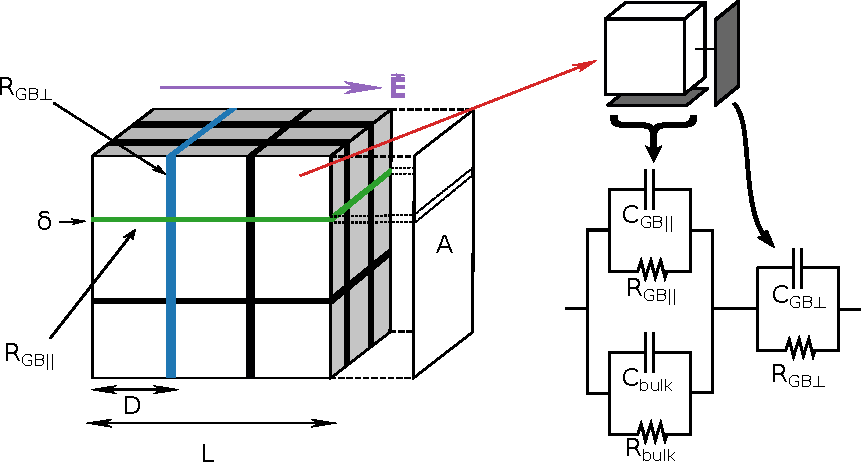
\includegraphics{Figures/brickLayerModel.pdf}
    \caption{The brick layer model with relevant dimensions and accompanying equivalent circuits.}
    \label{fig:appd:a:bricklayermodel}
\end{figure}
What follows is an explanation of the brick layer model that follows closely the work of Haile \cite{Haile1998}, N\"{a}fe \cite{Nafe1984}, and MacDonald \cite{Barsoukov2005}. This is here as a review and clarification of their arguments, and a derivation for the relevant parts of this dissertation. The conclusions of this model are widely used throughout the literature with little citation to the clearest explanation \cite{Bohn2000, Hossain2018, Chen2011}, so it may be useful to future students of EIS and solid oxide conductors.

The objective of the brick layer model is to create an electrical equivalent circuit that corresponds to the physical parameters of the sample itself, so that the impedance results can be used to calculate accurately the conductivities of the different regions of a polycrystalline sample. The two mechanisms considered here are that of the bulk grain interior ($\sigma_{\mathrm{bulk}}$) and that of the grain boundaries ($\sigma_{\mathrm{gb}}$). The impedance of these mechanisms differ over frequency and manifest in two semi-circular arcs in the Nyquist plot as see in the Figure \ref{meth:fig:eis:nyquist:ysz}. These characteristic frequencies ($\omega_0$) are attributed to the two conduction mechanisms by assigning the high frequency arc to the bulk conductivity and the mid frequency arc to the grain boundary conductivity (in principle the lowest frequency arc is attributed to the electrode response, but for simplicity it is omitted here). It is this assignment of bulk and grain boundary conduction to high and mid frequency response that we consider with the brick layer model here. 

There are three elements which need combining to form the brick layer model: the bulk resistance within the grains $R_{\mathrm{bulk}}$, the resistance of grain boundaries that run parallel to the applied electric field $R_{\mathrm{gb,}\parallel}$, and the resistance of grain boundaries that are oriented perpendicular to the applied electric field $R_{\mathrm{gb,}\perp}$. When considered this way it is easy to see that the bulk resistance and parallel grain boundaries are ``in parallel'' to each other, while they are together ``in series'' with the perpendicular grain boundaries. Thus $R_1$ from Figure \ref{fig:meth:RCRCmodel} is really composed of a parallel combination of $R_{\mathrm{bulk}}$ and $R_{\mathrm{gb,}\parallel}$ which yields 
\begin{equation}
    \frac{1}{R_1}\ = \frac{1}{R_{\mathrm{bulk}}}+\frac{1}{R_{\mathrm{gb,}\parallel}}\,.
    \label{eq:appd:a:r1_inverse}
\end{equation}
The conductivity for any element is related to the resistance by $1/R_i=\sigma_i L_i/A_i$. Important to note here is that the geometry of the components for each resistance equation. The total length for the grain boundary region perpendicular to the current according to Figure \ref{fig:appd:a:bricklayermodel} would be the sum the $m$ grain boundaries of length $\delta$, which can be approximated under the assumption that the grain boundaries are small in comparison to the grains by 
\begin{equation*}
L_{\mathrm{gb,\perp}} = m\delta = \frac{L \delta}{D + \delta} \approx \dfrac{L\delta}{D},
\end{equation*}
while the area is the same as the entire group, $A$. For the region of the grain boundary running parallel to the current, the length would be the same $L$ as the groups length, but the cross-sectional area would be approximated under similar considerations of grain boundary size by 
\begin{equation*}
    A_{\mathrm{gb,\parallel}}=\frac{2\delta}{D}A.
\end{equation*}
So by applying these equations to equation \ref{eq:appd:a:r1_inverse} we get
\begin{equation}
    \frac{1}{R_1} = \sigma_{\mathrm{bulk}}\frac{A}{L}+\sigma_{\mathrm{gb}}\left(\frac{2\delta}{D}A\right)\frac{1}{L}
    \label{eq:appd:r1_inverse_from_sb_sgb}
\end{equation}
Similarly for the resistance of the grain boundary oriented perpendicularly to the current,
\begin{equation}
    \frac{1}{R_2} =\sigma_{\mathrm{gb}}A\left(\frac{D}{L\, \delta}\right)
    \label{eq:appd:r2_inverse_from_s_gb}
\end{equation}
So by using the macroscopic parameters of the sample $L$ and $A$ and the resistances $R_1$ and $R_2$ to find $\sigma_1$ and $\sigma_2$ e.g.
\begin{equation*}
    \sigma_1 = \frac{L}{A R_1} \hspace{.5cm} \sigma_2 = \frac{L}{A R_2},
\end{equation*}
then relationships from these to the grain boundary and grain bulk conductivities can be formed:
\begin{equation}
    \sigma_1=\sigma_{\mathrm{bulk}}+\frac{2\delta}{D}\sigma_{\mathrm{gb}}
    \label{eq:appd:s_1to_s_bulk}
\end{equation}
\begin{equation}
    \sigma_2 = \frac{D}{\delta}\sigma_{\mathrm{gb}}
    \label{eq:appd:s_2to_s_gb}
\end{equation}
With these two equations in hand, it is useful to consider one assumption of polycrystalline materials and then three limiting cases of the relationship of bulk to grain boundary conductivity. In reality, for dense polycrystalline materials the size of the grain is large in comparison to the size of the boundary region between grains. That is to say that $\delta/D<<1$. This experimental reality points toward to cases for the relationship between the conductivities.



In the first limiting case of $\sigma_{\mathrm{bulk}}>\sigma_{\mathrm{gb}}$, it is easy to see from the above assumption in the relative sizes of $\delta$ and $D$ that $\sigma_1 = \sigma_\mathrm{bulk}$. In fact even in cases where the conductivities are of similar magnitude, due to the differences in the geometry of the bulk and grain boundary paths, the error in attributing $\sigma_1$ to $\sigma_{\mathrm{bulk}}$ would be due to the factor of $\delta/D$, perhaps only a few percent. Now modifying equation \ref{eq:appd:a:r1_inverse} allows 
\begin{equation}
    R_1 \approx R_{\mathrm{bulk}} \text{ and } R_2 \approx R_{\mathrm{gb}}
    \label{eq:appd:r1_reducedTo_r_bulk}
\end{equation}

At this point nothing has indicated the frequency response of these two pathways, and how the arcs in the Nyquist plot can be attributed on a consistent basis. As defined in equation \ref{eq:meth:timeConstant} the characteristic frequency is $\omega_0 = 1/RC$. By applying combining the formula for resistance in a material with the formula for the capacitance of a parallel plate capacitor we get
\begin{equation}
    \omega_0 = \frac{1}{RC} = \frac{1}{\left(\dfrac{1}{\sigma} \dfrac{l'}{A'}\right)\left(\epsilon_r \epsilon_0 \dfrac{A'}{l'}\right)} = \frac{\sigma}{\epsilon_r \epsilon_0}
\end{equation}
Written in this way, it is easy to see that under this model, the characteristic frequency of each conduction pathway is independent of its size. If we write
\begin{equation*}
    \omega_1 = \frac{1}{R_{\mathrm{bulk}} C_{\mathrm{bulk}}} = \frac{\sigma_{\mathrm{bulk}}}{\epsilon_{r, \mathrm{bulk}} \epsilon_0}
\end{equation*}
\begin{equation*}
    \omega_2 = \frac{1}{R_{\mathrm{gb}} C_{\mathrm{gb}}} = \frac{\sigma_{\mathrm{gb}}}{\epsilon_{r, \mathrm{gb}} \epsilon_0}
\end{equation*}
The final crucial assumption of the brick layer model is that the relative permittivities between the grain bulk and grain boundaries are approximately equal, and that this makes the differences in conductivity the important factor in the differences in characteristic frequency and thus placement on the Nyquist plot. This means that the question of which response is measured at higher frequency is a question of which conduction mechanism has the higher conductivity. Under the condition that grain interiors have a higher conductivity than grain boundaries, two separate time constants will occur, and the resistance of higher frequency portion $R_1$ can be used to  calculated $\sigma_{\mathrm{bulk}}$ directly from the geometrical parameters of the sample. The lower frequency arc $R_2$ will then be attributed to the conduction of the grain boundaries oriented perpendicular to the current.


The next limiting case to evaluate is when $\sigma_{\mathrm{bulk}}\approx \sigma_{\mathrm{gb}}$. Considering the importance of the fact that in order to have two distinguishable peaks, the values of characteristic frequency $\omega$ must be different by at least one order of magnitude, then with the same conductivity between grains and grain boundaries will produce only one peak in the Nyquist plot. Therefore resolving the differences between grain and grain boundary will be impossible. However, considering that the total resistance of the sample would be
\begin{equation}
    R_{\mathrm{total}} = R_1 + R_2 = R_1\left(1 + \frac{R_2}{R_1}\right)
    \label{eq:appd:totalResistance}
\end{equation}
and that the ratio of $R_2/R_1$ can be found from equations \ref{eq:appd:r1_inverse_from_sb_sgb} and \ref{eq:appd:r2_inverse_from_s_gb} as 
\begin{equation}
    \frac{R_2}{R_1} = \frac{\delta \sigma_{\mathrm{bulk}}}{D \sigma_{\mathrm{gb}}}+2\left(\frac{\delta}{D}\right)^2
\end{equation}
Since the ratio of $\delta/D$ is small this relationship shows that the resistance of this single arc that does appear will still be approximately equal to the resistance of the bulk. But no further information regarding the capacitances is possible. 



Finally, in the case of $\sigma_{\mathrm{bulk}}<\sigma_{\mathrm{gb}}$, because the conductivity of the grain boundary is higher than that of the grain interior it is possible to have a two arc response with the higher frequency arc attributed to grain boundaries. However, due to the size of the grain boundaries, and the need for the characteristic frequencies to be different by an order of magnitude, once these conditions are met the result is a high frequency arc that is very small in radius in comparison to the grain interior arc. The practical reality of being able to distinguish an arc that much smaller. As an example, for a sample even with grain boundary conductivity on the same order as grain bulk conductivity with a $\delta/D \approx 10^{-3}$, the resistances are different by three orders of magnitude. For higher conductivities this difference expands even more. Thus practically speaking only one arc will be present in the Nyquist plot.


As a result of the discussion, if two arcs are present in the Nyquist plot for a sample of typical microstructure, it is reasonable to conclude that the high frequency arc is the grain interior and the lower frequency arc from the grain boundary. By fitting the equivalent circuit and extracting parameters yield values for $R_1, R_2, C_1,$ and $C_2$.

Furthermore, using this assumption that the relative permittivities are approximately equal, allows another important simplification to be made. According to equation \ref{eq:appd:s_2to_s_gb} the conductivity of the grain boundary region can not be calculated without knowing the ratio of $D/\delta$. However by considering the parallel plate capacitor equations again in the context of knowing $\omega$ from the data as well as $R_1$ and $R_2$ then
\begin{equation*}
    C_1 = \frac{1}{R_1 \omega_1} = \epsilon_{r, \mathrm{bulk}} \epsilon_0 \frac{A}{L},
\end{equation*}
\begin{equation*}
    C_2 = \frac{1}{R_2 \omega_2} = \epsilon_{r, \mathrm{gb}} \epsilon_0 A \left(\frac{D}{L \delta}\right).
\end{equation*}
Dividing these equations and applying the assumption about equal relative permittivities, we get
\begin{equation}
    \frac{C_1}{C_2} = \frac{\delta}{D}.    
\end{equation}
This allows equation \ref{eq:appd:s_2to_s_gb} to be solved for $\sigma_{\mathrm{gb}}$ and written in terms of the capacitances,
\begin{equation}
    \sigma_{\mathrm{gb}} = \frac{\delta}{D} \sigma_2 = \frac{C_1}{C_2} \sigma_2
    \label{eq:appd:s_gb_approxWithCap12}
\end{equation}
Furthermore, since $\sigma_2$ was calculated with $L/AR_2$ then substitution into equation \ref{eq:appd:s_gb_approxWithCap12} yields a form found in much of the literature \cite{Gilardi2017}:
\begin{equation}
    \sigma_{\mathrm{gb}} = \frac{R_1 C_1}{R_2 C_2} \sigma_{\mathrm{bulk}} = \frac{\tau_1}{\tau_2}\sigma_{\mathrm{bulk}}
\end{equation}














